\vspace{-0.2cm}
\section{SFT on Self-Generated Data is Insufficient for Self-Correction}
\vspace{-0.2cm}
\label{sec:sft}

\begin{table}[t]
\centering
\caption{\footnotesize{\textbf{Self-correction performance after training on $\mathcal{D}_{\mathrm{STaR}}$ and $\mathcal{D}_{\mathrm{SFT}}$.} We find that the gap between the second and first attempts ($\Delta$(t1,t2)) is either negative or small. Both approaches erroneously modify a correct response to be incorrect, i.e., reflected in a high $\Delta^{\mathrm{c} \rightarrow \mathrm{i}}(t1, t2)$ and a low $\Delta^{\mathrm{i} \rightarrow \mathrm{c}}(t1, t2)$.}}
\label{tab:sft_results}
\renewcommand{\arraystretch}{1.25}
\resizebox{.9\textwidth}{!}{\begin{tabular}{lrrrrr}
\toprule
\textbf{Method}     & \textbf{Accuracy@t1} & \textbf{Accuracy@t2} & \textbf{$\Delta$(t1, t2)} & \textbf{$\Delta^{\mathrm{i} \rightarrow \mathrm{c}}$(t1, t2)} & \textbf{$\Delta^{\mathrm{c} \rightarrow \mathrm{i}}$(t1, t2)}  \\ \midrule
Base model & 52.6\%          & 41.4\%          & -11.2\%               & 4.6\%                & 15.8\%               \\ \midrule
STaR $\mathcal{D}_{\mathrm{StaR}}$      & 55.4\%          & 41.2\%          & -14.2\%                 & 5.4\%                  & 19.6\%                \\
STaR $\mathcal{D}_{\mathrm{StaR}}^+$     & 53.6\%          & 54.0\%          & 0.4\%                 & 2.6\%                  & 2.2\%                \\
\pairsft{} $\mathcal{D}_{\mathrm{SFT}}$       & 52.4\%          & 54.2\%          & 1.8\%                & 5.4\%                & 3.6\%                  \\
\pairsft{} $\mathcal{D}_{\mathrm{SFT}}^+$       & 55.0\%          & 55.0\%          & 0\%                & 0\%                & 0\%                  \\ \bottomrule
\end{tabular}}
\vspace{-0.2cm}
\end{table}

A natural approach for training self-correction is to utilize some form of supervised fine-tuning on data collected from a base model. Variants of this approach have been shown to scale well on single-turn reasoning problems~\citep{singh2023beyond, zelikman2022star}. In this section, we assess the empirical efficacy of two such approaches for self-correction: STaR~\citep{zelikman2022star}, and a version of \citet{welleck2023generating} that trains only one model. %

We ultimately find that although these methods improve self-correction over the base model, they fail to achieve substantially positive self-correction ($\Delta$\textbf{(t1,t2)}). By probing these models, we observe two main failure modes: \textbf{(1)} a collapse to non-correcting behavior, where the models learn to produce a good response on the first attempt and only make minor (or no) modifications in the second attempt, and \textbf{(2)} an inability of offline methods to be robust to distribution shift in the first-attempt responses. 




\textbf{Analysis setup: methods and dataset construction.} We prompt Gemini 1.5 Flash to obtain a large number of two-turn self-correction traces on MATH~\citep{hendrycksmath2021}. The \textbf{STaR} approach filters these trajectories to retain only those that successfully revise incorrect responses and runs SFT on the resulting dataset. Another approach is to use base model data from above to construct ``synthetic'' repair traces by pairing incorrect responses with correct ones~\citep{welleck2023generating}. We study a variant of this method that we call \textbf{\pairsft{}}, which does not train a separate corrector model and does not augment this initial dataset with multi-turn traces. Formally, we denote the datasets for STaR and \pairsft{} as $\mathcal{D}_{\mathrm{STaR}}$ and $\mathcal{D}_{\mathrm{SFT}}$ respectively. We run 3 iterations for STaR following the protocol in \citet{singh2024human}, and only one iteration for Pair-SFT, following the protocol in \citet{welleck2023generating} and other standard workflows on SFT.



\begin{figure}[t]
    \vspace{-0.2cm}
    \captionsetup{belowskip=-5pt}
    \centering
    \begin{minipage}{0.66\linewidth}
        \begin{subfigure}{\linewidth}
            \centering
            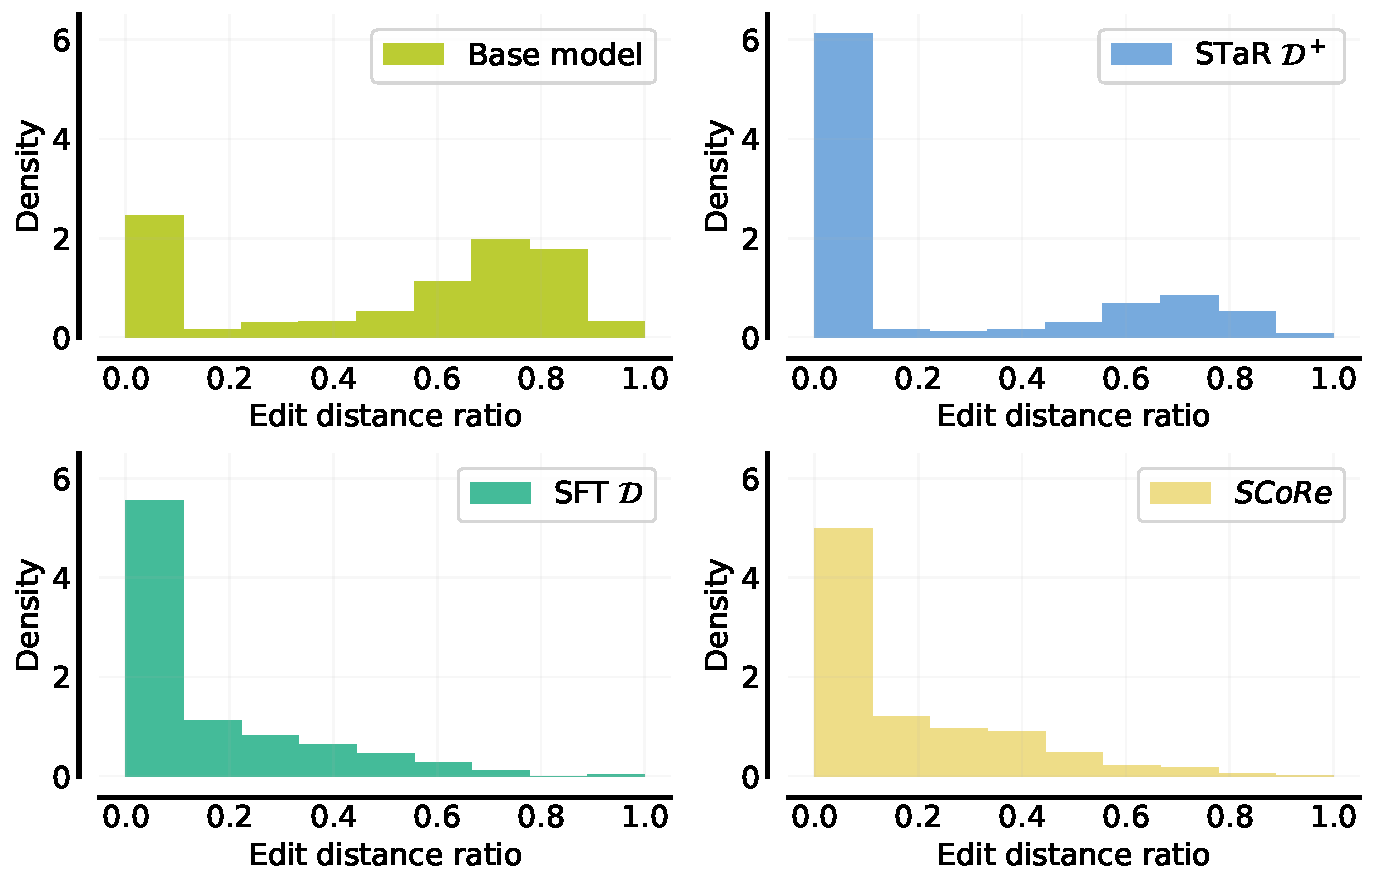
\includegraphics[width=\linewidth]{assets/edit_histogram_subplots.pdf}
            \caption{\footnotesize{\textbf{Histograms} of edit distance ratios on MATH 500.}}
            \label{fig:math_500_edit_ratios}
        \end{subfigure}
    \end{minipage}
    \begin{minipage}{.33\linewidth}
        \begin{subfigure}{\linewidth}
            \centering
            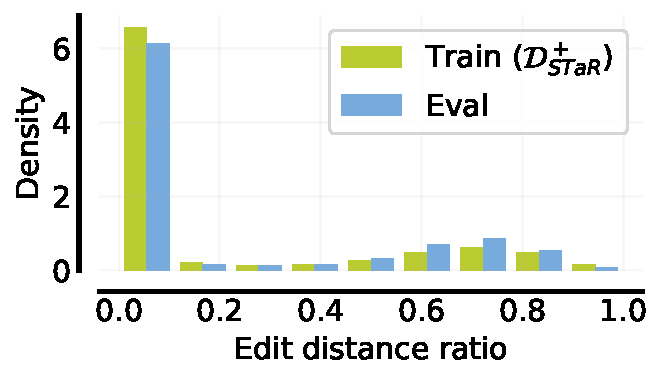
\includegraphics[width=\linewidth]{assets/star_edit_distances.pdf}
            \caption{\footnotesize{\textbf{STaR} edit distance ratios.}}
            \label{fig:star_ratios}
        \end{subfigure} \\[1ex]
        \begin{subfigure}{\linewidth}
            \centering
            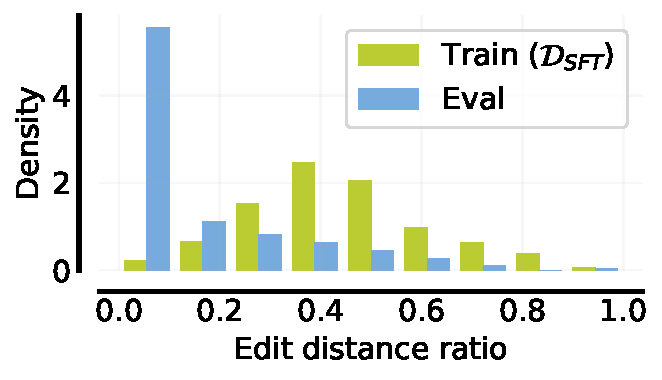
\includegraphics[width=\linewidth]{assets/sft_edit_distances.pdf}
            \caption{\footnotesize{\textbf{\pairsft} edit distance ratios.}}
            \label{fig:sft_ratios}
        \end{subfigure}
    \end{minipage}
    \caption{\footnotesize{\textbf{Edit distance between first-attempt and second-attempt responses} from fine-tuned models, our approach (\methodname{}) and the base model. While training on self-generated error correction traces learns to not make major edits primarily, SFT learns to make some edits but is still quite conservative.}}
    \vspace{-0.2cm}
\end{figure}

\begin{wrapfigure}{R}{0.57\linewidth}
    \vspace{-0.35cm}
    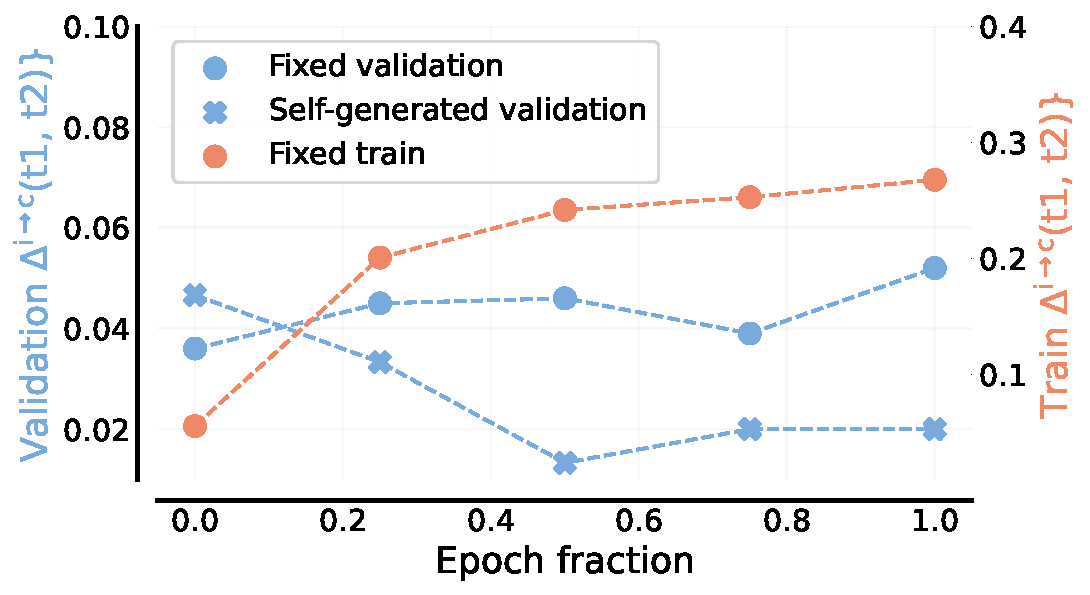
\includegraphics[width=0.99\linewidth]{assets/sft_validation.pdf}
    \vspace{-0.25cm}
    \caption{\label{fig:sft_validation}\footnotesize{\textbf{Self-correction performance} on different sets of first-attempt responses: (a) {``fixed''}: first response is sampled from the initial model, (b) ``self-generated'': first response is generated by the learner itself. Throughout training, the correction rate on fixed responses increases for both train and validation problems, but degrades substantially on self-generated responses. This indicates that training on a fixed offline dataset of correction traces suffers from distribution shift.}}
    \vspace{-0.2cm}
\end{wrapfigure}

\textbf{Main empirical findings.} We present the self-correction results before and after fine-tuning on $\mathcal{D}_{\mathrm{STaR}}$ and $\mathcal{D}_{\mathrm{SFT}}$ in Table~\ref{tab:sft_results}. We find that although $\Delta$\textbf{(t1, t2)} is substantially higher for \pairsft{} relative to the base model, there is only little benefit to self-correction (1.8\% gain). This gain is of a similar order to findings from \citet{qu2024recursive}. By studying $\icdelta$ and $\cidelta$, we find that SFT mainly reduces the number of correct problems that are mistakenly changed to incorrect in the second attempt, but does not significantly increase the fraction of incorrect first attempts that are corrected. This result is consistent with prior works on intrinsic self-correction that have found negligible or negative $\Delta$\textbf{(t1, t2)} values.

We also find that unlike \pairsft{}, training on $\mathcal{D}_{\mathrm{STaR}}$ does not reduce $\cidelta$, indicating that the STaR policy does not have a clear understanding of when to make modifications and when not to.
Observing this, we also trained on an extended version of $\mathcal{D}_{\mathrm{STaR}}^+$ (and $\mathcal{D}_{\mathrm{SFT}}^+$), which additionally contains tuples with both correct responses. We would expect the addition of such ``correct-to-correct'' data to prevent the model from erroneously revising a correct response. As shown in Table~\ref{tab:sft_results}, the inclusion of this data helps STaR substantially but only results in 0.4\%  change in $\Delta$\textbf{(t1, t2)}. On the other hand, for SFT, inclusion of this data overly biases the model against changing its answer.

\textbf{Diving deeper: analyzing self-correction behavior.} To further understand how these STaR and SFT models edit their responses, we measured their \textbf{edit distance ratios}, defined as the edit distance between the responses normalized by the total length of both the responses. As shown in Figure~\ref{fig:math_500_edit_ratios}, while the base model sometimes makes substantially large edits to the original response, models fine-tuned on $\mathcal{D}_{\mathrm{STaR}}$ and $\mathcal{D}_{\mathrm{SFT}}$ are overly conservative and often make no edits at all. This is akin to a form of \emph{\textbf{behavior collapse}}: training to maximize likelihoods on off-policy revision traces does not teach the desired correction ``behavior'', even though it improves first-attempt accuracy. Similar observations of LLMs ignoring nuanced behaviors (e.g., producing a mistake in a response and then correcting it in subsequent steps) have been observed in \citet{ye2024physicslanguagemodels22}. 

We also compared the distributions of edit distance ratios on training and test-time self-correction traces in Figures~\ref{fig:star_ratios}/\ref{fig:sft_ratios}. While STaR produces qualitatively similar edit distance ratios on both the train and validation sets, we still observe some discrepancies between the train and validation edit distance ratios for SFT, implying that \pairsft{} is not very effective at generalizing to new problems from the same distribution. We visualized this by plotting the self-correction performance of the SFT model on a fixed set of first attempts and self-generated first attempts in Figure~\ref{fig:sft_validation}. We observe vastly different behaviors between static and self-generated first-attempt distributions: while the model is able to optimize training correction accuracy and also slightly improves on first attempts appearing in the validation set (distributed \emph{i.i.d.} to the training distribution), its self-correction accuracy degrades. Hence, \emph{\textbf{distribution shift}} is a significant challenge for offline methods such as \pairsft{}.

\begin{AIbox}{Takeaways: Insufficiency of SFT}
SFT-based methods suffer from two distinct failures when learning self-correction: \textbf{(1)} distribution shift, and \textbf{(2)} behavior collapse. Training on on-policy data can fix \textbf{(1)}, but not \textbf{(2)}. 
\end{AIbox}








